\documentclass[11pt]{article}

    \usepackage[breakable]{tcolorbox}
    \usepackage{parskip} % Stop auto-indenting (to mimic markdown behaviour)
    
    \usepackage{iftex}
    \ifPDFTeX
    	\usepackage[T1]{fontenc}
    	\usepackage{mathpazo}
    \else
    	\usepackage{fontspec}
    \fi

    % Basic figure setup, for now with no caption control since it's done
    % automatically by Pandoc (which extracts ![](path) syntax from Markdown).
    \usepackage{graphicx}
    % Maintain compatibility with old templates. Remove in nbconvert 6.0
    \let\Oldincludegraphics\includegraphics
    % Ensure that by default, figures have no caption (until we provide a
    % proper Figure object with a Caption API and a way to capture that
    % in the conversion process - todo).
    \usepackage{caption}
    \DeclareCaptionFormat{nocaption}{}
    \captionsetup{format=nocaption,aboveskip=0pt,belowskip=0pt}

    \usepackage{float}
    \floatplacement{figure}{H} % forces figures to be placed at the correct location
    \usepackage{xcolor} % Allow colors to be defined
    \usepackage{enumerate} % Needed for markdown enumerations to work
    \usepackage{geometry} % Used to adjust the document margins
    \usepackage{amsmath} % Equations
    \usepackage{amssymb} % Equations
    \usepackage{textcomp} % defines textquotesingle
    % Hack from http://tex.stackexchange.com/a/47451/13684:
    \AtBeginDocument{%
        \def\PYZsq{\textquotesingle}% Upright quotes in Pygmentized code
    }
    \usepackage{upquote} % Upright quotes for verbatim code
    \usepackage{eurosym} % defines \euro
    \usepackage[mathletters]{ucs} % Extended unicode (utf-8) support
    \usepackage{fancyvrb} % verbatim replacement that allows latex
    \usepackage{grffile} % extends the file name processing of package graphics 
                         % to support a larger range
    \makeatletter % fix for old versions of grffile with XeLaTeX
    \@ifpackagelater{grffile}{2019/11/01}
    {
      % Do nothing on new versions
    }
    {
      \def\Gread@@xetex#1{%
        \IfFileExists{"\Gin@base".bb}%
        {\Gread@eps{\Gin@base.bb}}%
        {\Gread@@xetex@aux#1}%
      }
    }
    \makeatother
    \usepackage[Export]{adjustbox} % Used to constrain images to a maximum size
    \adjustboxset{max size={0.9\linewidth}{0.9\paperheight}}

    % The hyperref package gives us a pdf with properly built
    % internal navigation ('pdf bookmarks' for the table of contents,
    % internal cross-reference links, web links for URLs, etc.)
    \usepackage{hyperref}
    % The default LaTeX title has an obnoxious amount of whitespace. By default,
    % titling removes some of it. It also provides customization options.
    \usepackage{titling}
    \usepackage{longtable} % longtable support required by pandoc >1.10
    \usepackage{booktabs}  % table support for pandoc > 1.12.2
    \usepackage[inline]{enumitem} % IRkernel/repr support (it uses the enumerate* environment)
    \usepackage[normalem]{ulem} % ulem is needed to support strikethroughs (\sout)
                                % normalem makes italics be italics, not underlines
    \usepackage{mathrsfs}
    

    
    % Colors for the hyperref package
    \definecolor{urlcolor}{rgb}{0,.145,.698}
    \definecolor{linkcolor}{rgb}{.71,0.21,0.01}
    \definecolor{citecolor}{rgb}{.12,.54,.11}

    % ANSI colors
    \definecolor{ansi-black}{HTML}{3E424D}
    \definecolor{ansi-black-intense}{HTML}{282C36}
    \definecolor{ansi-red}{HTML}{E75C58}
    \definecolor{ansi-red-intense}{HTML}{B22B31}
    \definecolor{ansi-green}{HTML}{00A250}
    \definecolor{ansi-green-intense}{HTML}{007427}
    \definecolor{ansi-yellow}{HTML}{DDB62B}
    \definecolor{ansi-yellow-intense}{HTML}{B27D12}
    \definecolor{ansi-blue}{HTML}{208FFB}
    \definecolor{ansi-blue-intense}{HTML}{0065CA}
    \definecolor{ansi-magenta}{HTML}{D160C4}
    \definecolor{ansi-magenta-intense}{HTML}{A03196}
    \definecolor{ansi-cyan}{HTML}{60C6C8}
    \definecolor{ansi-cyan-intense}{HTML}{258F8F}
    \definecolor{ansi-white}{HTML}{C5C1B4}
    \definecolor{ansi-white-intense}{HTML}{A1A6B2}
    \definecolor{ansi-default-inverse-fg}{HTML}{FFFFFF}
    \definecolor{ansi-default-inverse-bg}{HTML}{000000}

    % common color for the border for error outputs.
    \definecolor{outerrorbackground}{HTML}{FFDFDF}

    % commands and environments needed by pandoc snippets
    % extracted from the output of `pandoc -s`
    \providecommand{\tightlist}{%
      \setlength{\itemsep}{0pt}\setlength{\parskip}{0pt}}
    \DefineVerbatimEnvironment{Highlighting}{Verbatim}{commandchars=\\\{\}}
    % Add ',fontsize=\small' for more characters per line
    \newenvironment{Shaded}{}{}
    \newcommand{\KeywordTok}[1]{\textcolor[rgb]{0.00,0.44,0.13}{\textbf{{#1}}}}
    \newcommand{\DataTypeTok}[1]{\textcolor[rgb]{0.56,0.13,0.00}{{#1}}}
    \newcommand{\DecValTok}[1]{\textcolor[rgb]{0.25,0.63,0.44}{{#1}}}
    \newcommand{\BaseNTok}[1]{\textcolor[rgb]{0.25,0.63,0.44}{{#1}}}
    \newcommand{\FloatTok}[1]{\textcolor[rgb]{0.25,0.63,0.44}{{#1}}}
    \newcommand{\CharTok}[1]{\textcolor[rgb]{0.25,0.44,0.63}{{#1}}}
    \newcommand{\StringTok}[1]{\textcolor[rgb]{0.25,0.44,0.63}{{#1}}}
    \newcommand{\CommentTok}[1]{\textcolor[rgb]{0.38,0.63,0.69}{\textit{{#1}}}}
    \newcommand{\OtherTok}[1]{\textcolor[rgb]{0.00,0.44,0.13}{{#1}}}
    \newcommand{\AlertTok}[1]{\textcolor[rgb]{1.00,0.00,0.00}{\textbf{{#1}}}}
    \newcommand{\FunctionTok}[1]{\textcolor[rgb]{0.02,0.16,0.49}{{#1}}}
    \newcommand{\RegionMarkerTok}[1]{{#1}}
    \newcommand{\ErrorTok}[1]{\textcolor[rgb]{1.00,0.00,0.00}{\textbf{{#1}}}}
    \newcommand{\NormalTok}[1]{{#1}}
    
    % Additional commands for more recent versions of Pandoc
    \newcommand{\ConstantTok}[1]{\textcolor[rgb]{0.53,0.00,0.00}{{#1}}}
    \newcommand{\SpecialCharTok}[1]{\textcolor[rgb]{0.25,0.44,0.63}{{#1}}}
    \newcommand{\VerbatimStringTok}[1]{\textcolor[rgb]{0.25,0.44,0.63}{{#1}}}
    \newcommand{\SpecialStringTok}[1]{\textcolor[rgb]{0.73,0.40,0.53}{{#1}}}
    \newcommand{\ImportTok}[1]{{#1}}
    \newcommand{\DocumentationTok}[1]{\textcolor[rgb]{0.73,0.13,0.13}{\textit{{#1}}}}
    \newcommand{\AnnotationTok}[1]{\textcolor[rgb]{0.38,0.63,0.69}{\textbf{\textit{{#1}}}}}
    \newcommand{\CommentVarTok}[1]{\textcolor[rgb]{0.38,0.63,0.69}{\textbf{\textit{{#1}}}}}
    \newcommand{\VariableTok}[1]{\textcolor[rgb]{0.10,0.09,0.49}{{#1}}}
    \newcommand{\ControlFlowTok}[1]{\textcolor[rgb]{0.00,0.44,0.13}{\textbf{{#1}}}}
    \newcommand{\OperatorTok}[1]{\textcolor[rgb]{0.40,0.40,0.40}{{#1}}}
    \newcommand{\BuiltInTok}[1]{{#1}}
    \newcommand{\ExtensionTok}[1]{{#1}}
    \newcommand{\PreprocessorTok}[1]{\textcolor[rgb]{0.74,0.48,0.00}{{#1}}}
    \newcommand{\AttributeTok}[1]{\textcolor[rgb]{0.49,0.56,0.16}{{#1}}}
    \newcommand{\InformationTok}[1]{\textcolor[rgb]{0.38,0.63,0.69}{\textbf{\textit{{#1}}}}}
    \newcommand{\WarningTok}[1]{\textcolor[rgb]{0.38,0.63,0.69}{\textbf{\textit{{#1}}}}}
    
    
    % Define a nice break command that doesn't care if a line doesn't already
    % exist.
    \def\br{\hspace*{\fill} \\* }
    % Math Jax compatibility definitions
    \def\gt{>}
    \def\lt{<}
    \let\Oldtex\TeX
    \let\Oldlatex\LaTeX
    \renewcommand{\TeX}{\textrm{\Oldtex}}
    \renewcommand{\LaTeX}{\textrm{\Oldlatex}}
    % Document parameters
    % Document title
    \title{3.1 Motion through pose composition}
    
    
    
    
    
% Pygments definitions
\makeatletter
\def\PY@reset{\let\PY@it=\relax \let\PY@bf=\relax%
    \let\PY@ul=\relax \let\PY@tc=\relax%
    \let\PY@bc=\relax \let\PY@ff=\relax}
\def\PY@tok#1{\csname PY@tok@#1\endcsname}
\def\PY@toks#1+{\ifx\relax#1\empty\else%
    \PY@tok{#1}\expandafter\PY@toks\fi}
\def\PY@do#1{\PY@bc{\PY@tc{\PY@ul{%
    \PY@it{\PY@bf{\PY@ff{#1}}}}}}}
\def\PY#1#2{\PY@reset\PY@toks#1+\relax+\PY@do{#2}}

\expandafter\def\csname PY@tok@w\endcsname{\def\PY@tc##1{\textcolor[rgb]{0.73,0.73,0.73}{##1}}}
\expandafter\def\csname PY@tok@c\endcsname{\let\PY@it=\textit\def\PY@tc##1{\textcolor[rgb]{0.25,0.50,0.50}{##1}}}
\expandafter\def\csname PY@tok@cp\endcsname{\def\PY@tc##1{\textcolor[rgb]{0.74,0.48,0.00}{##1}}}
\expandafter\def\csname PY@tok@k\endcsname{\let\PY@bf=\textbf\def\PY@tc##1{\textcolor[rgb]{0.00,0.50,0.00}{##1}}}
\expandafter\def\csname PY@tok@kp\endcsname{\def\PY@tc##1{\textcolor[rgb]{0.00,0.50,0.00}{##1}}}
\expandafter\def\csname PY@tok@kt\endcsname{\def\PY@tc##1{\textcolor[rgb]{0.69,0.00,0.25}{##1}}}
\expandafter\def\csname PY@tok@o\endcsname{\def\PY@tc##1{\textcolor[rgb]{0.40,0.40,0.40}{##1}}}
\expandafter\def\csname PY@tok@ow\endcsname{\let\PY@bf=\textbf\def\PY@tc##1{\textcolor[rgb]{0.67,0.13,1.00}{##1}}}
\expandafter\def\csname PY@tok@nb\endcsname{\def\PY@tc##1{\textcolor[rgb]{0.00,0.50,0.00}{##1}}}
\expandafter\def\csname PY@tok@nf\endcsname{\def\PY@tc##1{\textcolor[rgb]{0.00,0.00,1.00}{##1}}}
\expandafter\def\csname PY@tok@nc\endcsname{\let\PY@bf=\textbf\def\PY@tc##1{\textcolor[rgb]{0.00,0.00,1.00}{##1}}}
\expandafter\def\csname PY@tok@nn\endcsname{\let\PY@bf=\textbf\def\PY@tc##1{\textcolor[rgb]{0.00,0.00,1.00}{##1}}}
\expandafter\def\csname PY@tok@ne\endcsname{\let\PY@bf=\textbf\def\PY@tc##1{\textcolor[rgb]{0.82,0.25,0.23}{##1}}}
\expandafter\def\csname PY@tok@nv\endcsname{\def\PY@tc##1{\textcolor[rgb]{0.10,0.09,0.49}{##1}}}
\expandafter\def\csname PY@tok@no\endcsname{\def\PY@tc##1{\textcolor[rgb]{0.53,0.00,0.00}{##1}}}
\expandafter\def\csname PY@tok@nl\endcsname{\def\PY@tc##1{\textcolor[rgb]{0.63,0.63,0.00}{##1}}}
\expandafter\def\csname PY@tok@ni\endcsname{\let\PY@bf=\textbf\def\PY@tc##1{\textcolor[rgb]{0.60,0.60,0.60}{##1}}}
\expandafter\def\csname PY@tok@na\endcsname{\def\PY@tc##1{\textcolor[rgb]{0.49,0.56,0.16}{##1}}}
\expandafter\def\csname PY@tok@nt\endcsname{\let\PY@bf=\textbf\def\PY@tc##1{\textcolor[rgb]{0.00,0.50,0.00}{##1}}}
\expandafter\def\csname PY@tok@nd\endcsname{\def\PY@tc##1{\textcolor[rgb]{0.67,0.13,1.00}{##1}}}
\expandafter\def\csname PY@tok@s\endcsname{\def\PY@tc##1{\textcolor[rgb]{0.73,0.13,0.13}{##1}}}
\expandafter\def\csname PY@tok@sd\endcsname{\let\PY@it=\textit\def\PY@tc##1{\textcolor[rgb]{0.73,0.13,0.13}{##1}}}
\expandafter\def\csname PY@tok@si\endcsname{\let\PY@bf=\textbf\def\PY@tc##1{\textcolor[rgb]{0.73,0.40,0.53}{##1}}}
\expandafter\def\csname PY@tok@se\endcsname{\let\PY@bf=\textbf\def\PY@tc##1{\textcolor[rgb]{0.73,0.40,0.13}{##1}}}
\expandafter\def\csname PY@tok@sr\endcsname{\def\PY@tc##1{\textcolor[rgb]{0.73,0.40,0.53}{##1}}}
\expandafter\def\csname PY@tok@ss\endcsname{\def\PY@tc##1{\textcolor[rgb]{0.10,0.09,0.49}{##1}}}
\expandafter\def\csname PY@tok@sx\endcsname{\def\PY@tc##1{\textcolor[rgb]{0.00,0.50,0.00}{##1}}}
\expandafter\def\csname PY@tok@m\endcsname{\def\PY@tc##1{\textcolor[rgb]{0.40,0.40,0.40}{##1}}}
\expandafter\def\csname PY@tok@gh\endcsname{\let\PY@bf=\textbf\def\PY@tc##1{\textcolor[rgb]{0.00,0.00,0.50}{##1}}}
\expandafter\def\csname PY@tok@gu\endcsname{\let\PY@bf=\textbf\def\PY@tc##1{\textcolor[rgb]{0.50,0.00,0.50}{##1}}}
\expandafter\def\csname PY@tok@gd\endcsname{\def\PY@tc##1{\textcolor[rgb]{0.63,0.00,0.00}{##1}}}
\expandafter\def\csname PY@tok@gi\endcsname{\def\PY@tc##1{\textcolor[rgb]{0.00,0.63,0.00}{##1}}}
\expandafter\def\csname PY@tok@gr\endcsname{\def\PY@tc##1{\textcolor[rgb]{1.00,0.00,0.00}{##1}}}
\expandafter\def\csname PY@tok@ge\endcsname{\let\PY@it=\textit}
\expandafter\def\csname PY@tok@gs\endcsname{\let\PY@bf=\textbf}
\expandafter\def\csname PY@tok@gp\endcsname{\let\PY@bf=\textbf\def\PY@tc##1{\textcolor[rgb]{0.00,0.00,0.50}{##1}}}
\expandafter\def\csname PY@tok@go\endcsname{\def\PY@tc##1{\textcolor[rgb]{0.53,0.53,0.53}{##1}}}
\expandafter\def\csname PY@tok@gt\endcsname{\def\PY@tc##1{\textcolor[rgb]{0.00,0.27,0.87}{##1}}}
\expandafter\def\csname PY@tok@err\endcsname{\def\PY@bc##1{\setlength{\fboxsep}{0pt}\fcolorbox[rgb]{1.00,0.00,0.00}{1,1,1}{\strut ##1}}}
\expandafter\def\csname PY@tok@kc\endcsname{\let\PY@bf=\textbf\def\PY@tc##1{\textcolor[rgb]{0.00,0.50,0.00}{##1}}}
\expandafter\def\csname PY@tok@kd\endcsname{\let\PY@bf=\textbf\def\PY@tc##1{\textcolor[rgb]{0.00,0.50,0.00}{##1}}}
\expandafter\def\csname PY@tok@kn\endcsname{\let\PY@bf=\textbf\def\PY@tc##1{\textcolor[rgb]{0.00,0.50,0.00}{##1}}}
\expandafter\def\csname PY@tok@kr\endcsname{\let\PY@bf=\textbf\def\PY@tc##1{\textcolor[rgb]{0.00,0.50,0.00}{##1}}}
\expandafter\def\csname PY@tok@bp\endcsname{\def\PY@tc##1{\textcolor[rgb]{0.00,0.50,0.00}{##1}}}
\expandafter\def\csname PY@tok@fm\endcsname{\def\PY@tc##1{\textcolor[rgb]{0.00,0.00,1.00}{##1}}}
\expandafter\def\csname PY@tok@vc\endcsname{\def\PY@tc##1{\textcolor[rgb]{0.10,0.09,0.49}{##1}}}
\expandafter\def\csname PY@tok@vg\endcsname{\def\PY@tc##1{\textcolor[rgb]{0.10,0.09,0.49}{##1}}}
\expandafter\def\csname PY@tok@vi\endcsname{\def\PY@tc##1{\textcolor[rgb]{0.10,0.09,0.49}{##1}}}
\expandafter\def\csname PY@tok@vm\endcsname{\def\PY@tc##1{\textcolor[rgb]{0.10,0.09,0.49}{##1}}}
\expandafter\def\csname PY@tok@sa\endcsname{\def\PY@tc##1{\textcolor[rgb]{0.73,0.13,0.13}{##1}}}
\expandafter\def\csname PY@tok@sb\endcsname{\def\PY@tc##1{\textcolor[rgb]{0.73,0.13,0.13}{##1}}}
\expandafter\def\csname PY@tok@sc\endcsname{\def\PY@tc##1{\textcolor[rgb]{0.73,0.13,0.13}{##1}}}
\expandafter\def\csname PY@tok@dl\endcsname{\def\PY@tc##1{\textcolor[rgb]{0.73,0.13,0.13}{##1}}}
\expandafter\def\csname PY@tok@s2\endcsname{\def\PY@tc##1{\textcolor[rgb]{0.73,0.13,0.13}{##1}}}
\expandafter\def\csname PY@tok@sh\endcsname{\def\PY@tc##1{\textcolor[rgb]{0.73,0.13,0.13}{##1}}}
\expandafter\def\csname PY@tok@s1\endcsname{\def\PY@tc##1{\textcolor[rgb]{0.73,0.13,0.13}{##1}}}
\expandafter\def\csname PY@tok@mb\endcsname{\def\PY@tc##1{\textcolor[rgb]{0.40,0.40,0.40}{##1}}}
\expandafter\def\csname PY@tok@mf\endcsname{\def\PY@tc##1{\textcolor[rgb]{0.40,0.40,0.40}{##1}}}
\expandafter\def\csname PY@tok@mh\endcsname{\def\PY@tc##1{\textcolor[rgb]{0.40,0.40,0.40}{##1}}}
\expandafter\def\csname PY@tok@mi\endcsname{\def\PY@tc##1{\textcolor[rgb]{0.40,0.40,0.40}{##1}}}
\expandafter\def\csname PY@tok@il\endcsname{\def\PY@tc##1{\textcolor[rgb]{0.40,0.40,0.40}{##1}}}
\expandafter\def\csname PY@tok@mo\endcsname{\def\PY@tc##1{\textcolor[rgb]{0.40,0.40,0.40}{##1}}}
\expandafter\def\csname PY@tok@ch\endcsname{\let\PY@it=\textit\def\PY@tc##1{\textcolor[rgb]{0.25,0.50,0.50}{##1}}}
\expandafter\def\csname PY@tok@cm\endcsname{\let\PY@it=\textit\def\PY@tc##1{\textcolor[rgb]{0.25,0.50,0.50}{##1}}}
\expandafter\def\csname PY@tok@cpf\endcsname{\let\PY@it=\textit\def\PY@tc##1{\textcolor[rgb]{0.25,0.50,0.50}{##1}}}
\expandafter\def\csname PY@tok@c1\endcsname{\let\PY@it=\textit\def\PY@tc##1{\textcolor[rgb]{0.25,0.50,0.50}{##1}}}
\expandafter\def\csname PY@tok@cs\endcsname{\let\PY@it=\textit\def\PY@tc##1{\textcolor[rgb]{0.25,0.50,0.50}{##1}}}

\def\PYZbs{\char`\\}
\def\PYZus{\char`\_}
\def\PYZob{\char`\{}
\def\PYZcb{\char`\}}
\def\PYZca{\char`\^}
\def\PYZam{\char`\&}
\def\PYZlt{\char`\<}
\def\PYZgt{\char`\>}
\def\PYZsh{\char`\#}
\def\PYZpc{\char`\%}
\def\PYZdl{\char`\$}
\def\PYZhy{\char`\-}
\def\PYZsq{\char`\'}
\def\PYZdq{\char`\"}
\def\PYZti{\char`\~}
% for compatibility with earlier versions
\def\PYZat{@}
\def\PYZlb{[}
\def\PYZrb{]}
\makeatother


    % For linebreaks inside Verbatim environment from package fancyvrb. 
    \makeatletter
        \newbox\Wrappedcontinuationbox 
        \newbox\Wrappedvisiblespacebox 
        \newcommand*\Wrappedvisiblespace {\textcolor{red}{\textvisiblespace}} 
        \newcommand*\Wrappedcontinuationsymbol {\textcolor{red}{\llap{\tiny$\m@th\hookrightarrow$}}} 
        \newcommand*\Wrappedcontinuationindent {3ex } 
        \newcommand*\Wrappedafterbreak {\kern\Wrappedcontinuationindent\copy\Wrappedcontinuationbox} 
        % Take advantage of the already applied Pygments mark-up to insert 
        % potential linebreaks for TeX processing. 
        %        {, <, #, %, $, ' and ": go to next line. 
        %        _, }, ^, &, >, - and ~: stay at end of broken line. 
        % Use of \textquotesingle for straight quote. 
        \newcommand*\Wrappedbreaksatspecials {% 
            \def\PYGZus{\discretionary{\char`\_}{\Wrappedafterbreak}{\char`\_}}% 
            \def\PYGZob{\discretionary{}{\Wrappedafterbreak\char`\{}{\char`\{}}% 
            \def\PYGZcb{\discretionary{\char`\}}{\Wrappedafterbreak}{\char`\}}}% 
            \def\PYGZca{\discretionary{\char`\^}{\Wrappedafterbreak}{\char`\^}}% 
            \def\PYGZam{\discretionary{\char`\&}{\Wrappedafterbreak}{\char`\&}}% 
            \def\PYGZlt{\discretionary{}{\Wrappedafterbreak\char`\<}{\char`\<}}% 
            \def\PYGZgt{\discretionary{\char`\>}{\Wrappedafterbreak}{\char`\>}}% 
            \def\PYGZsh{\discretionary{}{\Wrappedafterbreak\char`\#}{\char`\#}}% 
            \def\PYGZpc{\discretionary{}{\Wrappedafterbreak\char`\%}{\char`\%}}% 
            \def\PYGZdl{\discretionary{}{\Wrappedafterbreak\char`\$}{\char`\$}}% 
            \def\PYGZhy{\discretionary{\char`\-}{\Wrappedafterbreak}{\char`\-}}% 
            \def\PYGZsq{\discretionary{}{\Wrappedafterbreak\textquotesingle}{\textquotesingle}}% 
            \def\PYGZdq{\discretionary{}{\Wrappedafterbreak\char`\"}{\char`\"}}% 
            \def\PYGZti{\discretionary{\char`\~}{\Wrappedafterbreak}{\char`\~}}% 
        } 
        % Some characters . , ; ? ! / are not pygmentized. 
        % This macro makes them "active" and they will insert potential linebreaks 
        \newcommand*\Wrappedbreaksatpunct {% 
            \lccode`\~`\.\lowercase{\def~}{\discretionary{\hbox{\char`\.}}{\Wrappedafterbreak}{\hbox{\char`\.}}}% 
            \lccode`\~`\,\lowercase{\def~}{\discretionary{\hbox{\char`\,}}{\Wrappedafterbreak}{\hbox{\char`\,}}}% 
            \lccode`\~`\;\lowercase{\def~}{\discretionary{\hbox{\char`\;}}{\Wrappedafterbreak}{\hbox{\char`\;}}}% 
            \lccode`\~`\:\lowercase{\def~}{\discretionary{\hbox{\char`\:}}{\Wrappedafterbreak}{\hbox{\char`\:}}}% 
            \lccode`\~`\?\lowercase{\def~}{\discretionary{\hbox{\char`\?}}{\Wrappedafterbreak}{\hbox{\char`\?}}}% 
            \lccode`\~`\!\lowercase{\def~}{\discretionary{\hbox{\char`\!}}{\Wrappedafterbreak}{\hbox{\char`\!}}}% 
            \lccode`\~`\/\lowercase{\def~}{\discretionary{\hbox{\char`\/}}{\Wrappedafterbreak}{\hbox{\char`\/}}}% 
            \catcode`\.\active
            \catcode`\,\active 
            \catcode`\;\active
            \catcode`\:\active
            \catcode`\?\active
            \catcode`\!\active
            \catcode`\/\active 
            \lccode`\~`\~ 	
        }
    \makeatother

    \let\OriginalVerbatim=\Verbatim
    \makeatletter
    \renewcommand{\Verbatim}[1][1]{%
        %\parskip\z@skip
        \sbox\Wrappedcontinuationbox {\Wrappedcontinuationsymbol}%
        \sbox\Wrappedvisiblespacebox {\FV@SetupFont\Wrappedvisiblespace}%
        \def\FancyVerbFormatLine ##1{\hsize\linewidth
            \vtop{\raggedright\hyphenpenalty\z@\exhyphenpenalty\z@
                \doublehyphendemerits\z@\finalhyphendemerits\z@
                \strut ##1\strut}%
        }%
        % If the linebreak is at a space, the latter will be displayed as visible
        % space at end of first line, and a continuation symbol starts next line.
        % Stretch/shrink are however usually zero for typewriter font.
        \def\FV@Space {%
            \nobreak\hskip\z@ plus\fontdimen3\font minus\fontdimen4\font
            \discretionary{\copy\Wrappedvisiblespacebox}{\Wrappedafterbreak}
            {\kern\fontdimen2\font}%
        }%
        
        % Allow breaks at special characters using \PYG... macros.
        \Wrappedbreaksatspecials
        % Breaks at punctuation characters . , ; ? ! and / need catcode=\active 	
        \OriginalVerbatim[#1,codes*=\Wrappedbreaksatpunct]%
    }
    \makeatother

    % Exact colors from NB
    \definecolor{incolor}{HTML}{303F9F}
    \definecolor{outcolor}{HTML}{D84315}
    \definecolor{cellborder}{HTML}{CFCFCF}
    \definecolor{cellbackground}{HTML}{F7F7F7}
    
    % prompt
    \makeatletter
    \newcommand{\boxspacing}{\kern\kvtcb@left@rule\kern\kvtcb@boxsep}
    \makeatother
    \newcommand{\prompt}[4]{
        {\ttfamily\llap{{\color{#2}[#3]:\hspace{3pt}#4}}\vspace{-\baselineskip}}
    }
    

    
    % Prevent overflowing lines due to hard-to-break entities
    \sloppy 
    % Setup hyperref package
    \hypersetup{
      breaklinks=true,  % so long urls are correctly broken across lines
      colorlinks=true,
      urlcolor=urlcolor,
      linkcolor=linkcolor,
      citecolor=citecolor,
      }
    % Slightly bigger margins than the latex defaults
    
    \geometry{verbose,tmargin=1in,bmargin=1in,lmargin=1in,rmargin=1in}
    
    

\begin{document}
    
    \maketitle
    
    

    
    \hypertarget{motion-through-pose-composition}{%
\section{3.1 Motion through pose
composition}\label{motion-through-pose-composition}}

A fundamental aspect of the development of mobile robots is the motion
itself. This is not a trivial matter, as many sources of motion error
appear: - wheel slippage, - inaccurate calibration, - limited resolution
during integration (time increments, measurement resolution), or -
unequal floor, among others.

These factors introduce uncertainty in the robot motion. Additionally,
other constraints to the movement difficult its implementation. This
particular chapter explores the concept of \emph{robot's pose} and how
we deal with it in a probabilistic context.

The pose itself can take multiple forms depending on the problem
context:

\begin{itemize}
\tightlist
\item
  \textbf{2D location}: In a planar context we only need to a 2d vector
  \([x, y]^T\) to locate a robot against a point of reference, the
  origin \((0, 0).\)
\item
  \textbf{2D pose}: In most cases involving mobile robots, the location
  alone is insufficient. We need an additional parameter known as
  orientation or \emph{bearing}. Therefore, a robot's pose is usually
  expressed as \([x, y, \theta]^T\) (see Fig. 1). \emph{In the rest of
  the book, we mostly refer to this one.}
\item
  \textbf{3D pose}: Although we will only mention it in passing, for
  robotics applications in the 3D space, \emph{i.e.} UAV or drones, not
  only a third axis \(z\) is added, but to handle the orientation in a
  3D environment we need 3 components, \emph{i.e.} roll, pitch and yaw.
  This course is centered around planar mobile robots so we will not use
  this one, nevertheless most methods could be adapted to 3D
  environments.
\end{itemize}

\begin{figure}
\centering
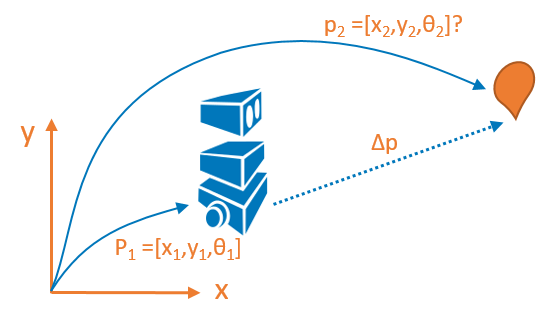
\includegraphics{images/pose-composition.png}
\end{figure}

Fig. 1: Example of an initial 2D robot pose (\(p_1\)) and its resultant
pose (\(p_2\)) after completing a motion (\(\Sigma p\)).

In this chapter we will explore how to use the \textbf{composition of
poses} to express poses in a certain reference system, while the next
two chapters describe two probabilistic methods for dealing with the
uncertainty inherent to robot motion, namely the \textbf{velocity-based}
motion model and the \textbf{odometry-based} one.

    \begin{tcolorbox}[breakable, size=fbox, boxrule=1pt, pad at break*=1mm,colback=cellbackground, colframe=cellborder]
\prompt{In}{incolor}{1}{\boxspacing}
\begin{Verbatim}[commandchars=\\\{\}]
\PY{o}{\PYZpc{}}\PY{k}{matplotlib} notebook

\PY{c+c1}{\PYZsh{} IMPORTS}

\PY{k+kn}{import} \PY{n+nn}{numpy} \PY{k}{as} \PY{n+nn}{np}
\PY{k+kn}{import} \PY{n+nn}{matplotlib}\PY{n+nn}{.}\PY{n+nn}{pyplot} \PY{k}{as} \PY{n+nn}{plt}
\PY{k+kn}{from} \PY{n+nn}{scipy} \PY{k+kn}{import} \PY{n}{stats}

\PY{k+kn}{import} \PY{n+nn}{sys}
\PY{n}{sys}\PY{o}{.}\PY{n}{path}\PY{o}{.}\PY{n}{append}\PY{p}{(}\PY{l+s+s2}{\PYZdq{}}\PY{l+s+s2}{..}\PY{l+s+s2}{\PYZdq{}}\PY{p}{)}
\PY{k+kn}{from} \PY{n+nn}{utils}\PY{n+nn}{.}\PY{n+nn}{DrawRobot} \PY{k+kn}{import} \PY{n}{DrawRobot}
\PY{k+kn}{from} \PY{n+nn}{utils}\PY{n+nn}{.}\PY{n+nn}{tcomp} \PY{k+kn}{import} \PY{n}{tcomp}
\end{Verbatim}
\end{tcolorbox}

    \hypertarget{optional}{%
\subsection{\texorpdfstring{{OPTIONAL}}{OPTIONAL}}\label{optional}}

{In the Robot motion lecture, we started talking about
\emph{Differential drive} motion systems. Include as many cells as
needed to introduce the background that you find interesting about it
and some code illustrating some related aspect, for example, a code
computing and plotting the \emph{Instantaneus Center of Rotation (ICR)}
according to a number of given parameters.}

    {\textbf{\emph{END OF OPTIONAL PART}}}

    \hypertarget{pose-composition}{%
\subsection{\texorpdfstring{3.1 Pose composition
}{3.1 Pose composition }}\label{pose-composition}}

The composition of posses is a tool that permits us to express the
\emph{final} pose of a robot in an arbitrary coordinate system. Given an
initial pose \(p_1\) and a pose differential \(\Delta p\), \emph{i.e.}
how much the robot has moved during an interval of time, we compute the
final pose \(p\) using the \textbf{composition of poses} function:

\[
    p_1 = 
        \begin{bmatrix}
            x_1 \\ y_1 \\ \theta_1
        \end{bmatrix}, \, \, \,
    \Delta p = 
        \begin{bmatrix}
            \Delta x \\ \Delta y \\ \Delta \theta
        \end{bmatrix}
\]

\[
    \begin{equation}
    p = \begin{bmatrix}
            x \\ y \\ \theta
        \end{bmatrix}
        = p_1 \oplus \Delta p
        = \begin{bmatrix}
            x_1 + \Delta x \cos \theta_1 - \Delta y \sin \theta_1 \\ 
            y_1 + \Delta x \sin \theta_1 + \Delta y \cos \theta_1 \\
            \theta_1 + \Delta \theta
          \end{bmatrix}
    \end{equation}
\]

The differential \(\Delta p\), although we are using it as control in
this exercise, normally is calculated given the robot's locomotion or
sensed by the wheel encoders.

    \hypertarget{optional}{%
\subsection{\texorpdfstring{{OPTIONAL}}{OPTIONAL}}\label{optional}}

{Implement your own methods to compute the composition of two poses, as
well as the inverse composition. Include some examples of their
utilization, also incorporating plots.}

    \begin{tcolorbox}[breakable, size=fbox, boxrule=1pt, pad at break*=1mm,colback=cellbackground, colframe=cellborder]
\prompt{In}{incolor}{2}{\boxspacing}
\begin{Verbatim}[commandchars=\\\{\}]
\PY{k}{def} \PY{n+nf}{composition}\PY{p}{(}\PY{n}{p1}\PY{p}{,}\PY{n}{p12}\PY{p}{)}\PY{p}{:}
    
    \PY{n}{p2} \PY{o}{=} \PY{n}{np}\PY{o}{.}\PY{n}{vstack}\PY{p}{(}\PY{p}{[}\PY{l+m+mf}{0.}\PY{p}{,}\PY{l+m+mf}{0.}\PY{p}{,}\PY{l+m+mf}{0.}\PY{p}{]}\PY{p}{)}

    \PY{n}{p2}\PY{p}{[}\PY{l+m+mi}{0}\PY{p}{,}\PY{l+m+mi}{0}\PY{p}{]} \PY{o}{=} \PY{n}{p1}\PY{p}{[}\PY{l+m+mi}{0}\PY{p}{,}\PY{l+m+mi}{0}\PY{p}{]} \PY{o}{+} \PY{n}{p12}\PY{p}{[}\PY{l+m+mi}{0}\PY{p}{,}\PY{l+m+mi}{0}\PY{p}{]}\PY{o}{*}\PY{n}{np}\PY{o}{.}\PY{n}{cos}\PY{p}{(}\PY{n}{p1}\PY{p}{[}\PY{l+m+mi}{2}\PY{p}{,} \PY{l+m+mi}{0}\PY{p}{]}\PY{p}{)} \PY{o}{\PYZhy{}} \PY{n}{p12}\PY{p}{[}\PY{l+m+mi}{1}\PY{p}{,}\PY{l+m+mi}{0}\PY{p}{]}\PY{o}{*}\PY{n}{np}\PY{o}{.}\PY{n}{sin}\PY{p}{(}\PY{n}{p1}\PY{p}{[}\PY{l+m+mi}{2}\PY{p}{,}\PY{l+m+mi}{0}\PY{p}{]}\PY{p}{)}
    \PY{n}{p2}\PY{p}{[}\PY{l+m+mi}{1}\PY{p}{,}\PY{l+m+mi}{0}\PY{p}{]} \PY{o}{=} \PY{n}{p1}\PY{p}{[}\PY{l+m+mi}{1}\PY{p}{,}\PY{l+m+mi}{0}\PY{p}{]} \PY{o}{+} \PY{n}{p12}\PY{p}{[}\PY{l+m+mi}{0}\PY{p}{,}\PY{l+m+mi}{0}\PY{p}{]}\PY{o}{*}\PY{n}{np}\PY{o}{.}\PY{n}{sin}\PY{p}{(}\PY{n}{p1}\PY{p}{[}\PY{l+m+mi}{2}\PY{p}{,} \PY{l+m+mi}{0}\PY{p}{]}\PY{p}{)} \PY{o}{+} \PY{n}{p12}\PY{p}{[}\PY{l+m+mi}{1}\PY{p}{,}\PY{l+m+mi}{0}\PY{p}{]}\PY{o}{*}\PY{n}{np}\PY{o}{.}\PY{n}{cos}\PY{p}{(}\PY{n}{p1}\PY{p}{[}\PY{l+m+mi}{2}\PY{p}{,}\PY{l+m+mi}{0}\PY{p}{]}\PY{p}{)}
   
    \PY{n}{p2}\PY{p}{[}\PY{l+m+mi}{2}\PY{p}{,}\PY{l+m+mi}{0}\PY{p}{]} \PY{o}{=} \PY{n}{p1}\PY{p}{[}\PY{l+m+mi}{2}\PY{p}{,}\PY{l+m+mi}{0}\PY{p}{]} \PY{o}{+} \PY{n}{p12}\PY{p}{[}\PY{l+m+mi}{2}\PY{p}{,}\PY{l+m+mi}{0}\PY{p}{]}

    \PY{c+c1}{\PYZsh{} Work with angle on range [0, 2*pi] rad}
    \PY{n}{p2}\PY{p}{[}\PY{l+m+mi}{2}\PY{p}{,}\PY{l+m+mi}{0}\PY{p}{]} \PY{o}{=} \PY{n}{p2}\PY{p}{[}\PY{l+m+mi}{2}\PY{p}{,}\PY{l+m+mi}{0}\PY{p}{]} \PY{o}{\PYZpc{}} \PY{p}{(}\PY{l+m+mi}{2}\PY{o}{*}\PY{n}{np}\PY{o}{.}\PY{n}{pi}\PY{p}{)}

    \PY{k}{return} \PY{n}{p2}
\end{Verbatim}
\end{tcolorbox}

    \begin{tcolorbox}[breakable, size=fbox, boxrule=1pt, pad at break*=1mm,colback=cellbackground, colframe=cellborder]
\prompt{In}{incolor}{3}{\boxspacing}
\begin{Verbatim}[commandchars=\\\{\}]
\PY{k}{def} \PY{n+nf}{inverseComposition}\PY{p}{(}\PY{n}{p1}\PY{p}{,} \PY{n}{p2}\PY{p}{)}\PY{p}{:}
    
    \PY{n}{p12} \PY{o}{=} \PY{n}{np}\PY{o}{.}\PY{n}{vstack}\PY{p}{(}\PY{p}{[}\PY{l+m+mf}{0.}\PY{p}{,}\PY{l+m+mf}{0.}\PY{p}{,}\PY{l+m+mf}{0.}\PY{p}{]}\PY{p}{)}

    \PY{n}{p12}\PY{p}{[}\PY{l+m+mi}{0}\PY{p}{,}\PY{l+m+mi}{0}\PY{p}{]} \PY{o}{=}  \PY{p}{(}\PY{n}{p2}\PY{p}{[}\PY{l+m+mi}{0}\PY{p}{,}\PY{l+m+mi}{0}\PY{p}{]}\PY{o}{\PYZhy{}}\PY{n}{p1}\PY{p}{[}\PY{l+m+mi}{0}\PY{p}{,}\PY{l+m+mi}{0}\PY{p}{]}\PY{p}{)}\PY{o}{*}\PY{n}{np}\PY{o}{.}\PY{n}{cos}\PY{p}{(}\PY{n}{p1}\PY{p}{[}\PY{l+m+mi}{2}\PY{p}{,} \PY{l+m+mi}{0}\PY{p}{]}\PY{p}{)} \PY{o}{+} \PY{p}{(}\PY{n}{p2}\PY{p}{[}\PY{l+m+mi}{1}\PY{p}{,}\PY{l+m+mi}{0}\PY{p}{]}\PY{o}{\PYZhy{}}\PY{n}{p1}\PY{p}{[}\PY{l+m+mi}{1}\PY{p}{,}\PY{l+m+mi}{0}\PY{p}{]}\PY{p}{)}\PY{o}{*}\PY{n}{np}\PY{o}{.}\PY{n}{sin}\PY{p}{(}\PY{n}{p1}\PY{p}{[}\PY{l+m+mi}{2}\PY{p}{,}\PY{l+m+mi}{0}\PY{p}{]}\PY{p}{)}
    \PY{n}{p12}\PY{p}{[}\PY{l+m+mi}{1}\PY{p}{,}\PY{l+m+mi}{0}\PY{p}{]} \PY{o}{=} \PY{o}{\PYZhy{}}\PY{p}{(}\PY{n}{p2}\PY{p}{[}\PY{l+m+mi}{0}\PY{p}{,}\PY{l+m+mi}{0}\PY{p}{]}\PY{o}{\PYZhy{}}\PY{n}{p1}\PY{p}{[}\PY{l+m+mi}{0}\PY{p}{,}\PY{l+m+mi}{0}\PY{p}{]}\PY{p}{)}\PY{o}{*}\PY{n}{np}\PY{o}{.}\PY{n}{sin}\PY{p}{(}\PY{n}{p1}\PY{p}{[}\PY{l+m+mi}{2}\PY{p}{,} \PY{l+m+mi}{0}\PY{p}{]}\PY{p}{)} \PY{o}{+} \PY{p}{(}\PY{n}{p2}\PY{p}{[}\PY{l+m+mi}{1}\PY{p}{,}\PY{l+m+mi}{0}\PY{p}{]}\PY{o}{\PYZhy{}}\PY{n}{p1}\PY{p}{[}\PY{l+m+mi}{1}\PY{p}{,}\PY{l+m+mi}{0}\PY{p}{]}\PY{p}{)}\PY{o}{*}\PY{n}{np}\PY{o}{.}\PY{n}{cos}\PY{p}{(}\PY{n}{p1}\PY{p}{[}\PY{l+m+mi}{2}\PY{p}{,}\PY{l+m+mi}{0}\PY{p}{]}\PY{p}{)}
   
    \PY{n}{p12}\PY{p}{[}\PY{l+m+mi}{2}\PY{p}{,}\PY{l+m+mi}{0}\PY{p}{]} \PY{o}{=} \PY{n}{p2}\PY{p}{[}\PY{l+m+mi}{2}\PY{p}{,}\PY{l+m+mi}{0}\PY{p}{]} \PY{o}{\PYZhy{}} \PY{n}{p1}\PY{p}{[}\PY{l+m+mi}{2}\PY{p}{,}\PY{l+m+mi}{0}\PY{p}{]}

    \PY{c+c1}{\PYZsh{} Work with angle on range [0, 2*pi] rad}
    \PY{n}{p12}\PY{p}{[}\PY{l+m+mi}{2}\PY{p}{,}\PY{l+m+mi}{0}\PY{p}{]} \PY{o}{=} \PY{n}{p12}\PY{p}{[}\PY{l+m+mi}{2}\PY{p}{,}\PY{l+m+mi}{0}\PY{p}{]} \PY{o}{\PYZpc{}} \PY{p}{(}\PY{l+m+mi}{2}\PY{o}{*}\PY{n}{np}\PY{o}{.}\PY{n}{pi}\PY{p}{)}

    \PY{k}{return} \PY{n}{p12}
\end{Verbatim}
\end{tcolorbox}

    \begin{tcolorbox}[breakable, size=fbox, boxrule=1pt, pad at break*=1mm,colback=cellbackground, colframe=cellborder]
\prompt{In}{incolor}{4}{\boxspacing}
\begin{Verbatim}[commandchars=\\\{\}]
\PY{k}{def} \PY{n+nf}{inversePose}\PY{p}{(}\PY{n}{p}\PY{p}{)}\PY{p}{:}
    
    \PY{n}{p\PYZus{}} \PY{o}{=} \PY{n}{np}\PY{o}{.}\PY{n}{vstack}\PY{p}{(}\PY{p}{[}\PY{l+m+mf}{0.}\PY{p}{,}\PY{l+m+mf}{0.}\PY{p}{,}\PY{l+m+mf}{0.}\PY{p}{]}\PY{p}{)}
    
    \PY{n}{p\PYZus{}}\PY{p}{[}\PY{l+m+mi}{0}\PY{p}{,}\PY{l+m+mi}{0}\PY{p}{]} \PY{o}{=}  \PY{o}{\PYZhy{}}\PY{n}{p}\PY{p}{[}\PY{l+m+mi}{0}\PY{p}{,}\PY{l+m+mi}{0}\PY{p}{]}\PY{o}{*}\PY{n}{np}\PY{o}{.}\PY{n}{cos}\PY{p}{(}\PY{n}{p}\PY{p}{[}\PY{l+m+mi}{2}\PY{p}{,}\PY{l+m+mi}{0}\PY{p}{]}\PY{p}{)} \PY{o}{\PYZhy{}} \PY{n}{p}\PY{p}{[}\PY{l+m+mi}{1}\PY{p}{,}\PY{l+m+mi}{0}\PY{p}{]}\PY{o}{*}\PY{n}{np}\PY{o}{.}\PY{n}{sin}\PY{p}{(}\PY{n}{p}\PY{p}{[}\PY{l+m+mi}{2}\PY{p}{,}\PY{l+m+mi}{0}\PY{p}{]}\PY{p}{)}
    \PY{n}{p\PYZus{}}\PY{p}{[}\PY{l+m+mi}{1}\PY{p}{,}\PY{l+m+mi}{0}\PY{p}{]} \PY{o}{=}   \PY{n}{p}\PY{p}{[}\PY{l+m+mi}{0}\PY{p}{,}\PY{l+m+mi}{0}\PY{p}{]}\PY{o}{*}\PY{n}{np}\PY{o}{.}\PY{n}{sin}\PY{p}{(}\PY{n}{p}\PY{p}{[}\PY{l+m+mi}{2}\PY{p}{,}\PY{l+m+mi}{0}\PY{p}{]}\PY{p}{)} \PY{o}{\PYZhy{}} \PY{n}{p}\PY{p}{[}\PY{l+m+mi}{1}\PY{p}{,}\PY{l+m+mi}{0}\PY{p}{]}\PY{o}{*}\PY{n}{np}\PY{o}{.}\PY{n}{cos}\PY{p}{(}\PY{n}{p}\PY{p}{[}\PY{l+m+mi}{2}\PY{p}{,}\PY{l+m+mi}{0}\PY{p}{]}\PY{p}{)}
   
    \PY{n}{p\PYZus{}}\PY{p}{[}\PY{l+m+mi}{2}\PY{p}{,}\PY{l+m+mi}{0}\PY{p}{]} \PY{o}{=} \PY{p}{(}\PY{o}{\PYZhy{}}\PY{n}{p}\PY{p}{[}\PY{l+m+mi}{2}\PY{p}{,}\PY{l+m+mi}{0}\PY{p}{]}\PY{p}{)} \PY{o}{\PYZpc{}} \PY{p}{(}\PY{l+m+mi}{2}\PY{o}{*}\PY{n}{np}\PY{o}{.}\PY{n}{pi}\PY{p}{)} \PY{c+c1}{\PYZsh{} Work with angle on range [0, 2*pi] rad}

    \PY{k}{return} \PY{n}{p\PYZus{}}
\end{Verbatim}
\end{tcolorbox}

    \begin{tcolorbox}[breakable, size=fbox, boxrule=1pt, pad at break*=1mm,colback=cellbackground, colframe=cellborder]
\prompt{In}{incolor}{5}{\boxspacing}
\begin{Verbatim}[commandchars=\\\{\}]
\PY{k}{def} \PY{n+nf}{compInv}\PY{p}{(}\PY{n}{p1}\PY{p}{,}\PY{n}{p2}\PY{p}{)}\PY{p}{:}
    \PY{k}{return} \PY{n}{composition}\PY{p}{(}\PY{n}{inversePose}\PY{p}{(}\PY{n}{p1}\PY{p}{)}\PY{p}{,}\PY{n}{p2}\PY{p}{)}
\end{Verbatim}
\end{tcolorbox}

    \begin{tcolorbox}[breakable, size=fbox, boxrule=1pt, pad at break*=1mm,colback=cellbackground, colframe=cellborder]
\prompt{In}{incolor}{7}{\boxspacing}
\begin{Verbatim}[commandchars=\\\{\}]
\PY{c+c1}{\PYZsh{}\PYZsh{}\PYZsh{}\PYZsh{}\PYZsh{}\PYZsh{}\PYZsh{}\PYZsh{}\PYZsh{}\PYZsh{}\PYZsh{}\PYZsh{}\PYZsh{}\PYZsh{}\PYZsh{}\PYZsh{}\PYZsh{}\PYZsh{}\PYZsh{}\PYZsh{}\PYZsh{}\PYZsh{}\PYZsh{}\PYZsh{}\PYZsh{}\PYZsh{}\PYZsh{}\PYZsh{}\PYZsh{}\PYZsh{}\PYZsh{}\PYZsh{}\PYZsh{}\PYZsh{}}
\PY{c+c1}{\PYZsh{} First, execute the class Robot \PYZsh{}}
\PY{c+c1}{\PYZsh{}\PYZsh{}\PYZsh{}\PYZsh{}\PYZsh{}\PYZsh{}\PYZsh{}\PYZsh{}\PYZsh{}\PYZsh{}\PYZsh{}\PYZsh{}\PYZsh{}\PYZsh{}\PYZsh{}\PYZsh{}\PYZsh{}\PYZsh{}\PYZsh{}\PYZsh{}\PYZsh{}\PYZsh{}\PYZsh{}\PYZsh{}\PYZsh{}\PYZsh{}\PYZsh{}\PYZsh{}\PYZsh{}\PYZsh{}\PYZsh{}\PYZsh{}\PYZsh{}\PYZsh{}}

\PY{n}{p1} \PY{o}{=} \PY{n}{np}\PY{o}{.}\PY{n}{vstack}\PY{p}{(}\PY{p}{[}\PY{l+m+mi}{1}\PY{p}{,} \PY{l+m+mi}{1}\PY{p}{,} \PY{n}{np}\PY{o}{.}\PY{n}{pi}\PY{o}{/}\PY{l+m+mi}{4}\PY{p}{]}\PY{p}{)}
\PY{n}{p12} \PY{o}{=} \PY{n}{np}\PY{o}{.}\PY{n}{vstack}\PY{p}{(}\PY{p}{[}\PY{l+m+mi}{3}\PY{o}{*}\PY{n}{np}\PY{o}{.}\PY{n}{sqrt}\PY{p}{(}\PY{l+m+mi}{2}\PY{p}{)}\PY{o}{/}\PY{l+m+mi}{2}\PY{p}{,} \PY{n}{np}\PY{o}{.}\PY{n}{sqrt}\PY{p}{(}\PY{l+m+mi}{2}\PY{p}{)}\PY{o}{/}\PY{l+m+mi}{2}\PY{p}{,} \PY{l+m+mi}{2}\PY{o}{*}\PY{n}{np}\PY{o}{.}\PY{n}{pi}\PY{o}{\PYZhy{}}\PY{n}{np}\PY{o}{.}\PY{n}{pi}\PY{o}{/}\PY{l+m+mi}{4}\PY{p}{]}\PY{p}{)}
\PY{n}{p23} \PY{o}{=} \PY{n}{np}\PY{o}{.}\PY{n}{vstack}\PY{p}{(}\PY{p}{[}\PY{l+m+mi}{1}\PY{p}{,} \PY{o}{\PYZhy{}}\PY{l+m+mi}{1}\PY{p}{,} \PY{l+m+mi}{0}\PY{p}{]}\PY{p}{)}

\PY{n}{p2} \PY{o}{=} \PY{n}{composition}\PY{p}{(}\PY{n}{p1}\PY{p}{,} \PY{n}{p12}\PY{p}{)}
\PY{n}{p3} \PY{o}{=} \PY{n}{composition}\PY{p}{(}\PY{n}{p2}\PY{p}{,} \PY{n}{p23}\PY{p}{)}

\PY{n}{p13} \PY{o}{=} \PY{n}{compInv}\PY{p}{(}\PY{n}{p1}\PY{p}{,} \PY{n}{p3}\PY{p}{)} \PY{c+c1}{\PYZsh{}?}

\PY{n}{p1\PYZus{}} \PY{o}{=} \PY{n}{inversePose}\PY{p}{(}\PY{n}{p1}\PY{p}{)}
\PY{n}{p2\PYZus{}} \PY{o}{=} \PY{n}{inversePose}\PY{p}{(}\PY{n}{p2}\PY{p}{)}
\PY{n}{p3\PYZus{}} \PY{o}{=} \PY{n}{inversePose}\PY{p}{(}\PY{n}{p3}\PY{p}{)}

\PY{n}{robot} \PY{o}{=} \PY{n}{Robot}\PY{p}{(}\PY{n}{p1}\PY{p}{)}
\PY{n}{robot2} \PY{o}{=} \PY{n}{Robot}\PY{p}{(}\PY{n}{p2}\PY{p}{)}
\PY{n}{robot3} \PY{o}{=} \PY{n}{Robot}\PY{p}{(}\PY{n}{p3}\PY{p}{)}

\PY{c+c1}{\PYZsh{} VISUALIZATION}
\PY{n}{fig}\PY{p}{,} \PY{n}{ax} \PY{o}{=} \PY{n}{plt}\PY{o}{.}\PY{n}{subplots}\PY{p}{(}\PY{p}{)}
\PY{n}{plt}\PY{o}{.}\PY{n}{ion}\PY{p}{(}\PY{p}{)}
\PY{n}{plt}\PY{o}{.}\PY{n}{draw}\PY{p}{(}\PY{p}{)}
\PY{n}{plt}\PY{o}{.}\PY{n}{xlim}\PY{p}{(}\PY{p}{(}\PY{l+m+mi}{0}\PY{p}{,} \PY{l+m+mi}{4}\PY{p}{)}\PY{p}{)}
\PY{n}{plt}\PY{o}{.}\PY{n}{ylim}\PY{p}{(}\PY{p}{(}\PY{l+m+mi}{0}\PY{p}{,} \PY{l+m+mi}{4}\PY{p}{)}\PY{p}{)}
\PY{n}{plt}\PY{o}{.}\PY{n}{grid}\PY{p}{(}\PY{p}{)}

\PY{n}{robot}\PY{o}{.}\PY{n}{draw}\PY{p}{(}\PY{n}{fig}\PY{p}{,} \PY{n}{ax}\PY{p}{,} \PY{l+s+s2}{\PYZdq{}}\PY{l+s+s2}{red}\PY{l+s+s2}{\PYZdq{}}\PY{p}{)}
\PY{n}{robot2}\PY{o}{.}\PY{n}{draw}\PY{p}{(}\PY{n}{fig}\PY{p}{,} \PY{n}{ax}\PY{p}{,} \PY{l+s+s2}{\PYZdq{}}\PY{l+s+s2}{blue}\PY{l+s+s2}{\PYZdq{}}\PY{p}{)}
\PY{n}{robot3}\PY{o}{.}\PY{n}{draw}\PY{p}{(}\PY{n}{fig}\PY{p}{,} \PY{n}{ax}\PY{p}{,} \PY{l+s+s2}{\PYZdq{}}\PY{l+s+s2}{green}\PY{l+s+s2}{\PYZdq{}}\PY{p}{)}

\PY{n+nb}{print}\PY{p}{(}\PY{l+s+s2}{\PYZdq{}}\PY{l+s+s2}{p1 \PYZhy{}\PYZgt{} }\PY{l+s+s2}{\PYZdq{}}\PY{p}{,} \PY{n}{p1}\PY{o}{.}\PY{n}{flatten}\PY{p}{(}\PY{p}{)}\PY{p}{,} \PY{l+s+s2}{\PYZdq{}}\PY{l+s+se}{\PYZbs{}n}\PY{l+s+s2}{p2 \PYZhy{}\PYZgt{} }\PY{l+s+s2}{\PYZdq{}}\PY{p}{,} \PY{n}{p2}\PY{o}{.}\PY{n}{flatten}\PY{p}{(}\PY{p}{)}\PY{p}{,}\PY{l+s+s2}{\PYZdq{}}\PY{l+s+se}{\PYZbs{}n}\PY{l+s+s2}{p3 \PYZhy{}\PYZgt{} }\PY{l+s+s2}{\PYZdq{}}\PY{p}{,} \PY{n}{p3}\PY{o}{.}\PY{n}{flatten}\PY{p}{(}\PY{p}{)}\PY{p}{,}\PY{l+s+s2}{\PYZdq{}}\PY{l+s+se}{\PYZbs{}n}\PY{l+s+s2}{\PYZdq{}}\PY{p}{)}
\PY{n+nb}{print}\PY{p}{(}\PY{l+s+s2}{\PYZdq{}}\PY{l+s+s2}{p12 \PYZhy{}\PYZgt{} }\PY{l+s+s2}{\PYZdq{}}\PY{p}{,} \PY{n}{p12}\PY{o}{.}\PY{n}{flatten}\PY{p}{(}\PY{p}{)}\PY{p}{,} \PY{l+s+s2}{\PYZdq{}}\PY{l+s+se}{\PYZbs{}n}\PY{l+s+s2}{p13 \PYZhy{}\PYZgt{} }\PY{l+s+s2}{\PYZdq{}}\PY{p}{,} \PY{n}{p13}\PY{o}{.}\PY{n}{flatten}\PY{p}{(}\PY{p}{)}\PY{p}{,}\PY{l+s+s2}{\PYZdq{}}\PY{l+s+se}{\PYZbs{}n}\PY{l+s+s2}{p23 \PYZhy{}\PYZgt{} }\PY{l+s+s2}{\PYZdq{}}\PY{p}{,} \PY{n}{p23}\PY{o}{.}\PY{n}{flatten}\PY{p}{(}\PY{p}{)}\PY{p}{,}\PY{l+s+s2}{\PYZdq{}}\PY{l+s+se}{\PYZbs{}n}\PY{l+s+s2}{\PYZdq{}}\PY{p}{)}
\PY{n+nb}{print}\PY{p}{(}\PY{l+s+s2}{\PYZdq{}}\PY{l+s+s2}{(\PYZhy{}p1 \PYZhy{}\PYZgt{} inverse of p1)}\PY{l+s+se}{\PYZbs{}n}\PY{l+s+s2}{\PYZdq{}}\PY{p}{)}
\PY{n+nb}{print}\PY{p}{(}\PY{l+s+s2}{\PYZdq{}}\PY{l+s+s2}{\PYZhy{}p1 \PYZhy{}\PYZgt{} }\PY{l+s+s2}{\PYZdq{}}\PY{p}{,} \PY{n}{p1\PYZus{}}\PY{o}{.}\PY{n}{flatten}\PY{p}{(}\PY{p}{)}\PY{p}{,} \PY{l+s+s2}{\PYZdq{}}\PY{l+s+se}{\PYZbs{}n}\PY{l+s+s2}{\PYZhy{}p2 \PYZhy{}\PYZgt{} }\PY{l+s+s2}{\PYZdq{}}\PY{p}{,} \PY{n}{p2\PYZus{}}\PY{o}{.}\PY{n}{flatten}\PY{p}{(}\PY{p}{)}\PY{p}{,}\PY{l+s+s2}{\PYZdq{}}\PY{l+s+se}{\PYZbs{}n}\PY{l+s+s2}{\PYZhy{}p3 \PYZhy{}\PYZgt{} }\PY{l+s+s2}{\PYZdq{}}\PY{p}{,} \PY{n}{p3\PYZus{}}\PY{o}{.}\PY{n}{flatten}\PY{p}{(}\PY{p}{)}\PY{p}{)}
\PY{n+nb}{print}\PY{p}{(}\PY{l+s+s2}{\PYZdq{}}\PY{l+s+se}{\PYZbs{}n}\PY{l+s+s2}{Null operation is satisfied:}\PY{l+s+se}{\PYZbs{}n}\PY{l+s+s2}{composition(\PYZhy{}p1,p1) = }\PY{l+s+s2}{\PYZdq{}}\PY{p}{,} \PY{n}{composition}\PY{p}{(}\PY{n}{p1\PYZus{}}\PY{p}{,} \PY{n}{p1}\PY{p}{)}\PY{o}{.}\PY{n}{flatten}\PY{p}{(}\PY{p}{)}\PY{p}{)}
\PY{n+nb}{print}\PY{p}{(}\PY{l+s+s2}{\PYZdq{}}\PY{l+s+se}{\PYZbs{}n}\PY{l+s+s2}{Null operation is satisfied:}\PY{l+s+se}{\PYZbs{}n}\PY{l+s+s2}{compInv(p1,p1) = }\PY{l+s+s2}{\PYZdq{}}\PY{p}{,} \PY{n}{compInv}\PY{p}{(}\PY{n}{p1}\PY{p}{,} \PY{n}{p1}\PY{p}{)}\PY{o}{.}\PY{n}{flatten}\PY{p}{(}\PY{p}{)}\PY{p}{)}
\PY{n+nb}{print}\PY{p}{(}\PY{l+s+s2}{\PYZdq{}}\PY{l+s+se}{\PYZbs{}n}\PY{l+s+s2}{Null operation is satisfied:}\PY{l+s+se}{\PYZbs{}n}\PY{l+s+s2}{inverseComposition(p1,p1) = }\PY{l+s+s2}{\PYZdq{}}\PY{p}{,} \PY{n}{inverseComposition}\PY{p}{(}\PY{n}{p1}\PY{p}{,} \PY{n}{p1}\PY{p}{)}\PY{o}{.}\PY{n}{flatten}\PY{p}{(}\PY{p}{)}\PY{p}{)}
\end{Verbatim}
\end{tcolorbox}

    
\begin{figure}
\centering
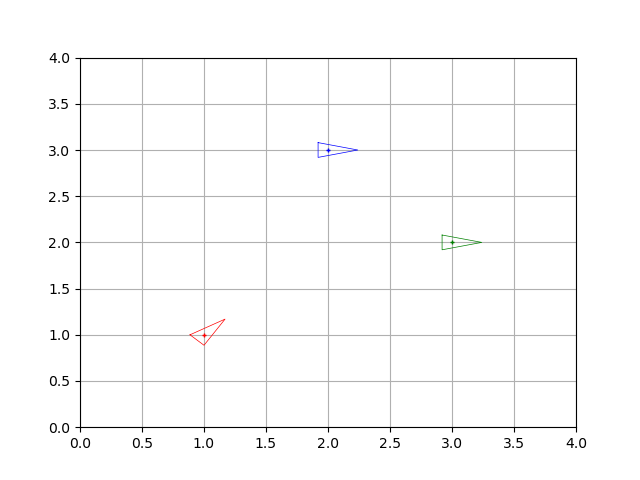
\includegraphics{returns/31opt.png}
\end{figure}

    
    \begin{Verbatim}[commandchars=\\\{\}]
p1 ->  [1.         1.         0.78539816]
p2 ->  [2. 3. 0.]
p3 ->  [3. 2. 0.]

p12 ->  [2.12132034 0.70710678 5.49778714]
p13 ->  [ 2.12132034 -0.70710678  5.49778714]
p23 ->  [ 1 -1  0]

(-p1 -> inverse of p1)

-p1 ->  [-1.41421356  0.          5.49778714]
-p2 ->  [-2. -3.  0.]
-p3 ->  [-3. -2.  0.]

Null operation is satisfied:
composition(-p1,p1) =  [-1.11022302e-16 -3.33066907e-16  0.00000000e+00]

Null operation is satisfied:
compInv(p1,p1) =  [-1.11022302e-16 -3.33066907e-16  0.00000000e+00]

Null operation is satisfied:
inverseComposition(p1,p1) =  [0. 0. 0.]
    \end{Verbatim}

    {\textbf{\emph{END OF OPTIONAL PART}}}

    \hypertarget{assignment-1-moving-the-robot-by-composing-pose-increments}{%
\subsubsection{\texorpdfstring{\textbf{{ASSIGNMENT 1: Moving the robot
by composing pose
increments}}}{ASSIGNMENT 1: Moving the robot by composing pose increments}}\label{assignment-1-moving-the-robot-by-composing-pose-increments}}

Take a look at the \texttt{Robot()} class provided and its methods: the
constructor, \texttt{step()} and \texttt{draw()}. Then, modify the main
function in the next cell for the robot to describe a \(8m \times 8m\)
square path as seen in the figure below. You must take into account
that:

\begin{itemize}
\tightlist
\item
  The robot starts in the bottom-left corner \((0, 0)\) heading north
  and
\item
  moves at increments of \(2 m\) each step.
\item
  Each 4 steps, it will turn right.
\end{itemize}

\textbf{Example}

\begin{figure}
\centering
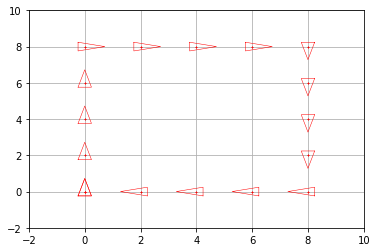
\includegraphics{images/fig3-1-1.png}
\end{figure}
Fig. 2: Route of our robot.

    \begin{tcolorbox}[breakable, size=fbox, boxrule=1pt, pad at break*=1mm,colback=cellbackground, colframe=cellborder]
\prompt{In}{incolor}{6}{\boxspacing}
\begin{Verbatim}[commandchars=\\\{\}]
\PY{k}{class} \PY{n+nc}{Robot}\PY{p}{(}\PY{p}{)}\PY{p}{:}
    \PY{l+s+sd}{\PYZsq{}\PYZsq{}\PYZsq{}Mobile robot implementation}
\PY{l+s+sd}{    }
\PY{l+s+sd}{        Attr:}
\PY{l+s+sd}{            pose: Expected position of the robot}
\PY{l+s+sd}{    \PYZsq{}\PYZsq{}\PYZsq{}}
    \PY{k}{def} \PY{n+nf+fm}{\PYZus{}\PYZus{}init\PYZus{}\PYZus{}}\PY{p}{(}\PY{n+nb+bp}{self}\PY{p}{,} \PY{n}{mean}\PY{p}{)}\PY{p}{:}
        \PY{n+nb+bp}{self}\PY{o}{.}\PY{n}{pose} \PY{o}{=} \PY{n}{mean}

    \PY{k}{def} \PY{n+nf}{step}\PY{p}{(}\PY{n+nb+bp}{self}\PY{p}{,} \PY{n}{u}\PY{p}{)}\PY{p}{:}
        \PY{n+nb+bp}{self}\PY{o}{.}\PY{n}{pose} \PY{o}{=} \PY{n}{tcomp}\PY{p}{(}\PY{n+nb+bp}{self}\PY{o}{.}\PY{n}{pose}\PY{p}{,} \PY{n}{u}\PY{p}{)}
    
    \PY{k}{def} \PY{n+nf}{draw}\PY{p}{(}\PY{n+nb+bp}{self}\PY{p}{,} \PY{n}{fig}\PY{p}{,} \PY{n}{ax}\PY{p}{,} \PY{n}{colour}\PY{o}{=}\PY{l+s+s2}{\PYZdq{}}\PY{l+s+s2}{red}\PY{l+s+s2}{\PYZdq{}}\PY{p}{)}\PY{p}{:}
        \PY{n}{DrawRobot}\PY{p}{(}\PY{n}{fig}\PY{p}{,} \PY{n}{ax}\PY{p}{,} \PY{n+nb+bp}{self}\PY{o}{.}\PY{n}{pose}\PY{p}{,} \PY{n}{color}\PY{o}{=}\PY{n}{colour}\PY{p}{)}
\end{Verbatim}
\end{tcolorbox}

    \begin{tcolorbox}[breakable, size=fbox, boxrule=1pt, pad at break*=1mm,colback=cellbackground, colframe=cellborder]
\prompt{In}{incolor}{8}{\boxspacing}
\begin{Verbatim}[commandchars=\\\{\}]
\PY{k}{def} \PY{n+nf}{main}\PY{p}{(}\PY{n}{robot}\PY{p}{)}\PY{p}{:}
    
    \PY{c+c1}{\PYZsh{} PARAMETERS INITIALIZATION}
    \PY{n}{num\PYZus{}steps} \PY{o}{=} \PY{l+m+mi}{15} \PY{c+c1}{\PYZsh{} Number of robot motions}
    \PY{n}{turning} \PY{o}{=} \PY{l+m+mi}{4}  \PY{c+c1}{\PYZsh{} Number of steps for turning}
    \PY{n}{u} \PY{o}{=} \PY{n}{np}\PY{o}{.}\PY{n}{vstack}\PY{p}{(}\PY{p}{[}\PY{l+m+mf}{2.}\PY{p}{,} \PY{l+m+mf}{0.}\PY{p}{,} \PY{l+m+mf}{0.}\PY{p}{]}\PY{p}{)} \PY{c+c1}{\PYZsh{} Motion command (pose increment)}
    \PY{n}{angle\PYZus{}inc} \PY{o}{=} \PY{o}{\PYZhy{}}\PY{n}{np}\PY{o}{.}\PY{n}{pi}\PY{o}{/}\PY{l+m+mi}{2} \PY{c+c1}{\PYZsh{} Angle increment}
    
    \PY{c+c1}{\PYZsh{} VISUALIZATION}
    \PY{n}{fig}\PY{p}{,} \PY{n}{ax} \PY{o}{=} \PY{n}{plt}\PY{o}{.}\PY{n}{subplots}\PY{p}{(}\PY{p}{)}
    \PY{n}{plt}\PY{o}{.}\PY{n}{ion}\PY{p}{(}\PY{p}{)}
    \PY{n}{plt}\PY{o}{.}\PY{n}{draw}\PY{p}{(}\PY{p}{)}
    \PY{n}{plt}\PY{o}{.}\PY{n}{xlim}\PY{p}{(}\PY{p}{(}\PY{o}{\PYZhy{}}\PY{l+m+mi}{2}\PY{p}{,} \PY{l+m+mi}{10}\PY{p}{)}\PY{p}{)}
    \PY{n}{plt}\PY{o}{.}\PY{n}{ylim}\PY{p}{(}\PY{p}{(}\PY{o}{\PYZhy{}}\PY{l+m+mi}{2}\PY{p}{,} \PY{l+m+mi}{10}\PY{p}{)}\PY{p}{)}
    
    \PY{n}{plt}\PY{o}{.}\PY{n}{grid}\PY{p}{(}\PY{p}{)}
    \PY{n}{robot}\PY{o}{.}\PY{n}{draw}\PY{p}{(}\PY{n}{fig}\PY{p}{,} \PY{n}{ax}\PY{p}{)}
    
    \PY{c+c1}{\PYZsh{} MAIN LOOP}
    \PY{k}{for} \PY{n}{step} \PY{o+ow}{in} \PY{n+nb}{range}\PY{p}{(}\PY{l+m+mi}{1}\PY{p}{,}\PY{n}{num\PYZus{}steps}\PY{o}{+}\PY{l+m+mi}{1}\PY{p}{)}\PY{p}{:}
        
        \PY{c+c1}{\PYZsh{} Check if the robot has to move in straight line or also has to turn}
        \PY{c+c1}{\PYZsh{} and accordingly set the third component (rotation) of the motion command }
        
        \PY{n}{turning} \PY{o}{=} \PY{n}{turning} \PY{o}{\PYZhy{}}\PY{l+m+mi}{1}
           
        \PY{k}{if} \PY{n}{turning} \PY{o}{==} \PY{l+m+mi}{0}\PY{p}{:}
            \PY{n}{u}\PY{p}{[}\PY{l+m+mi}{2}\PY{p}{]} \PY{o}{=} \PY{n}{u}\PY{p}{[}\PY{l+m+mi}{2}\PY{p}{]}\PY{o}{+}\PY{n}{angle\PYZus{}inc}
            \PY{n}{turning} \PY{o}{=} \PY{l+m+mi}{4}
        \PY{k}{else}\PY{p}{:}
            \PY{n}{u}\PY{p}{[}\PY{l+m+mi}{2}\PY{p}{]}\PY{o}{=}\PY{l+m+mi}{0}
            
        
        \PY{c+c1}{\PYZsh{} Execute the motion command        }
        \PY{n}{robot}\PY{o}{.}\PY{n}{step}\PY{p}{(}\PY{n}{u}\PY{p}{)}
        
        \PY{c+c1}{\PYZsh{} VISUALIZATION}
        \PY{n}{robot}\PY{o}{.}\PY{n}{draw}\PY{p}{(}\PY{n}{fig}\PY{p}{,} \PY{n}{ax}\PY{p}{)}
        \PY{n}{fig}\PY{o}{.}\PY{n}{canvas}\PY{o}{.}\PY{n}{draw}\PY{p}{(}\PY{p}{)}
        \PY{n}{plt}\PY{o}{.}\PY{n}{pause}\PY{p}{(}\PY{l+m+mf}{0.2}\PY{p}{)}   
    
\end{Verbatim}
\end{tcolorbox}

    Execute the following code cell to \textbf{try your code}. The resulting
figure must be the same as Fig. 2.

    \begin{tcolorbox}[breakable, size=fbox, boxrule=1pt, pad at break*=1mm,colback=cellbackground, colframe=cellborder]
\prompt{In}{incolor}{9}{\boxspacing}
\begin{Verbatim}[commandchars=\\\{\}]
\PY{c+c1}{\PYZsh{} RUN }
\PY{n}{initial\PYZus{}pose} \PY{o}{=} \PY{n}{np}\PY{o}{.}\PY{n}{vstack}\PY{p}{(}\PY{p}{[}\PY{l+m+mf}{0.}\PY{p}{,} \PY{l+m+mf}{0.}\PY{p}{,} \PY{n}{np}\PY{o}{.}\PY{n}{pi}\PY{o}{/}\PY{l+m+mi}{2}\PY{p}{]}\PY{p}{)}
\PY{n}{robot} \PY{o}{=} \PY{n}{Robot}\PY{p}{(}\PY{n}{initial\PYZus{}pose}\PY{p}{)}
\PY{n}{main}\PY{p}{(}\PY{n}{robot}\PY{p}{)}
\end{Verbatim}
\end{tcolorbox}

    
\begin{figure}
\centering
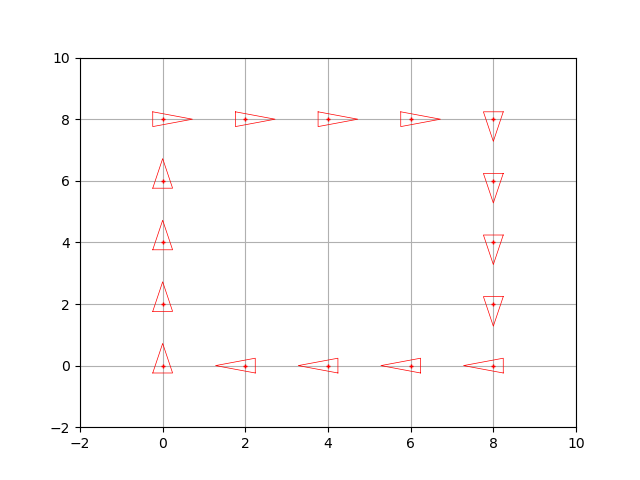
\includegraphics{returns/311.png}
\end{figure}

    
    \hypertarget{considering-noise}{%
\subsection{3.2 Considering noise}\label{considering-noise}}

In the previous case, the robot motion was error-free. This is overly
optimistic as in a real use case the conditions of the environment are a
huge source of uncertainty.

To take into consideration such uncertainty, we will model the movement
of the robot as a (multidimensional) gaussian distribution
\(\Delta p \sim N(\mu_{\Delta p},\Sigma_{\Delta p})\) where:

\begin{itemize}
\tightlist
\item
  The mean \(\mu_{\Delta p}\) is still the pose differential in the
  previous exercise, that is \(\Delta p_{\text{given}}\).
\item
  The covariance \(\Sigma_{\Delta p}\) is a \(3 \times 3\) matrix, which
  defines the amount of error at each step (time interval).
\end{itemize}

    \hypertarget{assignment-2-adding-noise-to-the-pose-motion}{%
\subsubsection{\texorpdfstring{\textbf{{ASSIGNMENT 2: Adding noise to
the pose
motion}}}{ASSIGNMENT 2: Adding noise to the pose motion}}\label{assignment-2-adding-noise-to-the-pose-motion}}

Now, we are going to add a Gaussian noise to the motion, assuming that
the incremental motion now follows the probability distribution:

\[
    \Delta p = N(\Delta p_{given}, \Sigma_{\Delta p})
    \textit{ with } 
    \Sigma_{\Delta p}  =
        \begin{bmatrix}
            0.04 & 0 & 0 \\
            0 & 0.04 & 0 \\
            0 & 0 & 0.01
        \end{bmatrix}
    (\text{ units in }m^2 \text{ and } rad^2)
\]

For doing that, complete the \texttt{NosyRobot()} class below, which is
a child class of the previous \texttt{Robot()} one. Concretely, you have
to:

\begin{itemize}
\tightlist
\item
  Complete this new class by adding some amount of noise to the movement
  (take a look at the \texttt{step()} method. \emph{Hints:
  \href{https://docs.scipy.org/doc/numpy/reference/generated/numpy.vstack.html}{\texttt{np.vstack()}},
  \href{https://docs.scipy.org/doc/scipy/reference/generated/scipy.stats.multivariate_normal.html}{\texttt{stats.multivariate\_normal.rvs()}}}.
  Remark that we have now two variables related to the robot pose:

  \begin{itemize}
  \tightlist
  \item
    \texttt{self.pose}, which represents the expected, \emph{ideal}
    pose, and
  \item
    \texttt{self.true\_pose}, that stands for the actual pose after
    carrying out a noisy motion command.
  \end{itemize}
\item
  Along with the expected pose drawn in red (\texttt{self.pose}), in the
  \texttt{draw()} method plot the real pose of the robot
  (\texttt{self.true\_pose}) in blue, which as commented is affected by
  noise.
\end{itemize}

Run the cell several times to see that the motion (and the path) is
different each time. Try also with different values of the covariance
matrix.

\textbf{Example}

\begin{figure}
\centering
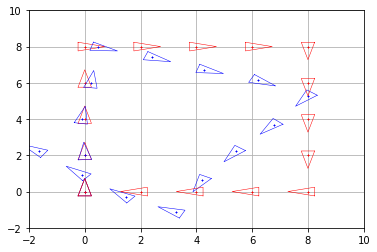
\includegraphics{images/fig3-1-2.png}
\end{figure}
Fig. 3: Movement of our robot using pose compositions. Containing the
expected poses (in red) and the true pose affected by noise (in blue)

    \begin{tcolorbox}[breakable, size=fbox, boxrule=1pt, pad at break*=1mm,colback=cellbackground, colframe=cellborder]
\prompt{In}{incolor}{10}{\boxspacing}
\begin{Verbatim}[commandchars=\\\{\}]
\PY{k}{class} \PY{n+nc}{NoisyRobot}\PY{p}{(}\PY{n}{Robot}\PY{p}{)}\PY{p}{:}
    \PY{l+s+sd}{\PYZdq{}\PYZdq{}\PYZdq{}Mobile robot implementation. It\PYZsq{}s motion has a set ammount of noise.}
\PY{l+s+sd}{    }
\PY{l+s+sd}{        Attr:}
\PY{l+s+sd}{            pose: Inherited from Robot}
\PY{l+s+sd}{            true\PYZus{}pose: Real robot pose, which has been affected by some ammount of noise.}
\PY{l+s+sd}{            covariance: Amount of error of each step.}
\PY{l+s+sd}{    \PYZdq{}\PYZdq{}\PYZdq{}}
    \PY{k}{def} \PY{n+nf+fm}{\PYZus{}\PYZus{}init\PYZus{}\PYZus{}}\PY{p}{(}\PY{n+nb+bp}{self}\PY{p}{,} \PY{n}{mean}\PY{p}{,} \PY{n}{covariance}\PY{p}{)}\PY{p}{:}
        \PY{n+nb}{super}\PY{p}{(}\PY{p}{)}\PY{o}{.}\PY{n+nf+fm}{\PYZus{}\PYZus{}init\PYZus{}\PYZus{}}\PY{p}{(}\PY{n}{mean}\PY{p}{)}
        \PY{n+nb+bp}{self}\PY{o}{.}\PY{n}{true\PYZus{}pose} \PY{o}{=} \PY{n}{mean}
        \PY{n+nb+bp}{self}\PY{o}{.}\PY{n}{covariance} \PY{o}{=} \PY{n}{covariance}
        
    \PY{k}{def} \PY{n+nf}{step}\PY{p}{(}\PY{n+nb+bp}{self}\PY{p}{,} \PY{n}{step\PYZus{}increment}\PY{p}{)}\PY{p}{:}
        \PY{l+s+sd}{\PYZdq{}\PYZdq{}\PYZdq{}Computes a single step of our noisy robot.}
\PY{l+s+sd}{        }
\PY{l+s+sd}{            super().step(...) updates the expected pose (without noise)}
\PY{l+s+sd}{            Generate a noisy increment based on step\PYZus{}increment and self.covariance.}
\PY{l+s+sd}{            Then this noisy increment is applied to self.true\PYZus{}pose}
\PY{l+s+sd}{        \PYZdq{}\PYZdq{}\PYZdq{}}
        \PY{n+nb}{super}\PY{p}{(}\PY{p}{)}\PY{o}{.}\PY{n}{step}\PY{p}{(}\PY{n}{step\PYZus{}increment}\PY{p}{)}
        
        \PY{n}{true\PYZus{}step} \PY{o}{=} \PY{n}{stats}\PY{o}{.}\PY{n}{multivariate\PYZus{}normal}\PY{o}{.}\PY{n}{rvs}\PY{p}{(}\PY{n}{step\PYZus{}increment}\PY{o}{.}\PY{n}{flatten}\PY{p}{(}\PY{p}{)}\PY{p}{,} \PY{n+nb+bp}{self}\PY{o}{.}\PY{n}{covariance}\PY{p}{)}
        \PY{n+nb+bp}{self}\PY{o}{.}\PY{n}{true\PYZus{}pose} \PY{o}{=} \PY{n}{tcomp}\PY{p}{(}\PY{n+nb+bp}{self}\PY{o}{.}\PY{n}{true\PYZus{}pose}\PY{p}{,} \PY{n}{np}\PY{o}{.}\PY{n}{vstack}\PY{p}{(}\PY{n}{true\PYZus{}step}\PY{p}{)}\PY{p}{)}
        
    \PY{k}{def} \PY{n+nf}{draw}\PY{p}{(}\PY{n+nb+bp}{self}\PY{p}{,} \PY{n}{fig}\PY{p}{,} \PY{n}{ax}\PY{p}{)}\PY{p}{:}
        \PY{n+nb}{super}\PY{p}{(}\PY{p}{)}\PY{o}{.}\PY{n}{draw}\PY{p}{(}\PY{n}{fig}\PY{p}{,} \PY{n}{ax}\PY{p}{)}
        \PY{n}{DrawRobot}\PY{p}{(}\PY{n}{fig}\PY{p}{,} \PY{n}{ax}\PY{p}{,} \PY{n+nb+bp}{self}\PY{o}{.}\PY{n}{true\PYZus{}pose}\PY{p}{,} \PY{n}{color}\PY{o}{=}\PY{l+s+s1}{\PYZsq{}}\PY{l+s+s1}{blue}\PY{l+s+s1}{\PYZsq{}}\PY{p}{)}
\end{Verbatim}
\end{tcolorbox}

    \begin{tcolorbox}[breakable, size=fbox, boxrule=1pt, pad at break*=1mm,colback=cellbackground, colframe=cellborder]
\prompt{In}{incolor}{21}{\boxspacing}
\begin{Verbatim}[commandchars=\\\{\}]
\PY{c+c1}{\PYZsh{} RUN }
\PY{n}{initial\PYZus{}pose} \PY{o}{=} \PY{n}{np}\PY{o}{.}\PY{n}{vstack}\PY{p}{(}\PY{p}{[}\PY{l+m+mf}{0.}\PY{p}{,} \PY{l+m+mf}{0.}\PY{p}{,} \PY{n}{np}\PY{o}{.}\PY{n}{pi}\PY{o}{/}\PY{l+m+mi}{2}\PY{p}{]}\PY{p}{)}
\PY{n}{cov} \PY{o}{=} \PY{n}{np}\PY{o}{.}\PY{n}{diag}\PY{p}{(}\PY{p}{[}\PY{l+m+mf}{0.04}\PY{p}{,} \PY{l+m+mf}{0.04}\PY{p}{,} \PY{l+m+mf}{0.01}\PY{p}{]}\PY{p}{)}  

\PY{n}{robot} \PY{o}{=} \PY{n}{NoisyRobot}\PY{p}{(}\PY{n}{initial\PYZus{}pose}\PY{p}{,} \PY{n}{cov}\PY{p}{)}
\PY{n}{main}\PY{p}{(}\PY{n}{robot}\PY{p}{)}
\end{Verbatim}
\end{tcolorbox}

\begin{figure}
\centering
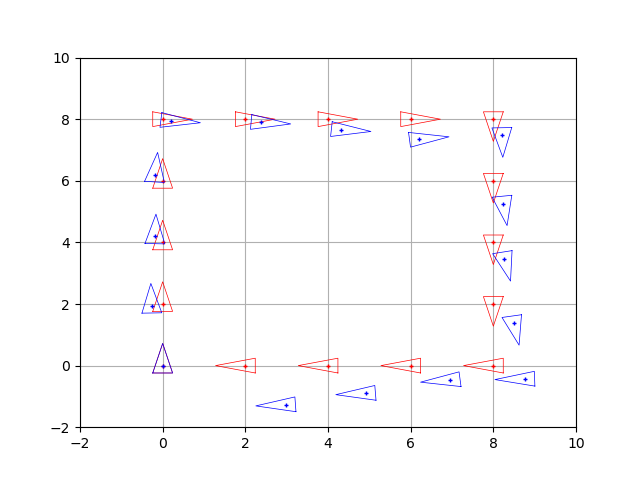
\includegraphics{returns/312.png}
\end{figure}
    
    \hypertarget{thinking-about-it-1}{%
\subsubsection{Thinking about it (1)}\label{thinking-about-it-1}}

Now that you are an expert in retrieving the pose of a robot after
carrying out a motion command defined as a pose increment,
\textbf{answer the following questions}:

\begin{itemize}
\item
  Why are the expected (blue) and true (red) poses different?

  Because the red pose is the expected and without errors pose and the
  blue one have some noise added.
\item
  In which scenario could they be the same?

  In the one which the random variable never introduces noise. (Pretty
  lucky)
\item
  How affect the values in the covariance matrix \(\Sigma_{\Delta p}\)
  the robot motion?

  When the diagonal values of the covariance matrix are higher, more
  dispersed could be our robot pose.
\end{itemize}


    % Add a bibliography block to the postdoc
    
    
    
\end{document}
